
%%%%%%%%%%%%%%%%
%%%%%%%%%%%%%%%%

\section{An improved DEC analysis} \label{sec:bg_epoch}

In this section, we'll focus on techniques that allow permit more realistic biogeographic analyses.
Topics include applying range size constraints, area connectivity, stratified/epoch models, function-valued dispersal rates, and incorporating uncertainty in paleogeographic event time estimates.
These modifications should produce more realistic ancestral range estimates, e.g. that a volcanic island may only be colonized once it has formed, and that distance should have some bearing on dispersal rate.

The remaining tutorials will make use of geographical and paleogeographical measurements for the Hawaiian archipelago, summarized in Table \ref{tab:paleogeo}.
Even though we will continue to use four areas (K, O, M, H) for Section \ref{sec:bg_epoch}, we will use all six areas (R, K, O, M, H, Z) in future sections, hence the full table is given for reference.
The paleogeographical information is encoded in the files named {\tt hawaii.n4.times.txt}, {\tt hawaii.n4.distances.txt}, and {\tt hawaii.n4.connectivity.*.txt}.

\begin{table}[!h]
\centering
\begin{tabular}{l|c|cc|cccccc}
area & code & $a_{max}$ & $a_{min}$ & $g_{\bullet R}$ & $g_{\bullet K}$ & $g_{\bullet O}$ & $g_{\bullet M}$ & $g_{\bullet H}$  & $g_{\bullet Z}$ \\ \hline
Older islands & R & - & - & - & 261 & 406 & 500 & 680 & 3900 \\
Kauai & K & 5.15 & 5.05 & - & - & 145 & 239 & 419 & 3900 \\
Oahu & O & 3.7  & 2.2  & - & -  & -  & 059 & 239 & 3900 \\
Maui Nui & M & 1.8  & 1.3  & - & -  & -  & -  & 082 & 3900 \\
Hawaii & H & 0.7  & 0.3  & - & -  & -  & -  & - & 3900 \\
Mainland & Z & - & - & - & - & - & - & - & - \\
\end{tabular}
\caption{Hawaiian paleogeography model. The six areas are given in Figure \ref{fig:hawaii_areas}.
Ages $a_{max}$ and $a_{min}$ report the maximum and minimum origination times for the given island.
Distances $g_{ij}$ report the shortest geographical distance from the coast of the row's area to the column's area (at present).}
\label{tab:paleogeo}
\end{table}

\subsection*{Analysis}

Start by creating our filename variables

\begin{snugshade}
\begin{lstlisting}
range_fn = "data/n4/silversword.n4.range.nex"
tree_fn = "data/n4/silversword.tre"
out_fn = "output/epoch"
geo_fn = "data/n4/hawaii.n4"
times_fn = geo_fn + ".times.txt"
dist_fn = geo_fn + ".distances.txt"
\end{lstlisting}
\end{snugshade}

Create some helper analysis variables

\begin{snugshade}
\begin{lstlisting}
mvi = 1
mni = 1
n_gen = 5000
\end{lstlisting}
\end{snugshade}


Read in the presence-absence range characters and record the number of areas in the dataset

\begin{snugshade}
\begin{lstlisting}
dat_range_01 = readDiscreteCharacterData(range_fn)
n_areas <- dat_range_01.nchar()
\end{lstlisting}
\end{snugshade}

Often, biogeographers wish to limit to the maximum allowable range size.
This prohibits widespread species ranges and to reduce the total number of range states in the analysis, thus benefitting computational efficiency.
Suppose we disallowed ranges from including more than two areas.
The total number of ranges equals $\sum_{k=0}^m {{n}\choose{k}}$ where $n$ is the total number of areas, $m$ is the maximum number of permissible areas, and ${{n}\choose{k}}$ is the number of ways to sample $k$ unordered areas from a pool of $n$ areas.

\begin{snugshade}
\begin{lstlisting}
max_areas <- 2
n_states <- 0
for (k in 0:max_areas) n_states += choose(n_areas, k)
\end{lstlisting}
\end{snugshade}

Then format the dataset for the reduced state space

\begin{snugshade}
\begin{lstlisting}
dat_range_n = formatDiscreteCharacterData(dat_range_01, "DEC", n_states)
\end{lstlisting}
\end{snugshade}

Our state space now includes only 11 states ($\emptyset$, K, O, M, H, KO, KM, OM, KH, OH, MH).

% read in some geography data
Next, we'll set up the paleogeographic model.
Read in the list of minimum and maximum ages of island formation

\begin{snugshade}
\begin{lstlisting}
time_bounds <- readDataDelimitedFile(file=times_fn, delimiter=" ")
n_epochs <- time_bounds.size()
\end{lstlisting}
\end{snugshade}

Read in a vector of matrices that describe the connectivity between areas over time.
Note, there is one connectivity matrix per epoch, ordered from oldest to youngest.

\begin{snugshade}
\begin{lstlisting}
for (i in 1:n_epochs) {
  epoch_fn[i] = geo_fn + ".connectivity." + i + ".txt"
  connectivity[i] <- readDataDelimitedFile(file=epoch_fn[i], delimiter=" ")
}
\end{lstlisting}
\end{snugshade}

Read in the matrix of distances between all pairs of areas (km). For simplicity, we will assume that distances remain constant over time, even though they certainly vary.

\begin{snugshade}
\begin{lstlisting}
distances <- readDataDelimitedFile(file=dist_fn, delimiter=" ")
\end{lstlisting}
\end{snugshade}


For now, we'll assume we know the dated species phylogeny without error.

\begin{snugshade}
\begin{lstlisting}
tree <- readTrees(tree_fn)[1]
\end{lstlisting}
\end{snugshade}

% distances between areas

Dispersal rates might make use of some extrinsic information, such as geographical distances between areas \citep{macarthur67, webb12}.
We model this as $d_{ij} = a e ^ {-b g_{ij}}$ where $g_{ij}$ is the geographical distance between areas $i$ and $j$ and $a$ and $b$ are parameters that scale distance on linear and exponential scales, respectively. Note that all dispersal rates equal $a$ when $b=0$.
The variables $a$, $b$, $d_{ij}$, and $g_{ij}$ are stored in memory as {\tt dispersal\_rate}, {\tt distance\_scale}, {\tt dr[i][j]}, and {\tt distances[i][j]}.

\begin{snugshade}
\begin{lstlisting}
log10_rate_bg ~ dnUniform(-4,2)
log10_rate_bg.setValue(-2)
rate_bg := 10^log10_rate_bg
moves[mvi++] = mvSlide(log10_rate_bg, weight=4)
\end{lstlisting}
\end{snugshade}

Fix the base dispersal rate to 1

\begin{snugshade}
\begin{lstlisting}
dispersal_rate <- abs(1)
\end{lstlisting}
\end{snugshade}

Add a distance scale parameter

\begin{snugshade}
\begin{lstlisting}
distance_scale ~ dnUnif(0,20)
distance_scale.setValue(0.01)
moves[mvi++] = mvScale(distance_scale, weight=3)
\end{lstlisting}
\end{snugshade}

Now we can assign rates that are functions of distance between all pairs of areas

%dr[i][j][k] := (a * exp( -b * distances[j][k] ))
\begin{snugshade}
\begin{lstlisting}
for (i in 1:n_epochs) {
  for (j in 1:n_areas) {
    for (k in 1:n_areas) {
      dr[i][j][k] <- abs(0)
      if (connectivity[i][j][k] > 0) {
        dr[i][j][k]  := dispersal_rate * exp(-distance_scale * distances[j][k])
      }
    }
  }
}
\end{lstlisting}
\end{snugshade}


% extirpation penalized ranges
% ... they can exist, but not persist

It is unlikely that widespread ranges persist across disjunct areas for long periods of time.
Extirpation is more likely to occur in fragmented ranges than well-connected ranges, where peripheral populations are continuously reinforced from the center.

\begin{snugshade}
\begin{lstlisting}
log_sd <- 0.5
log_mean <- ln(1) - 0.5*log_sd^2
extirpation_rate ~ dnLognormal(mean=log_mean, sd=log_sd)
moves[mvi++] = mvScale(extirpation_rate, weight=2)
\end{lstlisting}
\end{snugshade}

\begin{snugshade}
\begin{lstlisting}
for (i in 1:n_epochs) {
  for (j in 1:n_areas) {
    for (k in 1:n_areas) {
      er[i][j][k] <- abs(0.0) 
    }
    er[i][j][j] := extirpation_rate
  }
}
\end{lstlisting}
\end{snugshade}



Build a rate matrix for each time interval
\begin{snugshade}
\begin{lstlisting}
for (i in 1:n_epochs) {
  Q_DEC[i] := fnDECRateMatrix(dispersalRates=dr[i],
                              extirpationRates=er[i],
                              maxRangeSize=max_areas)
}
\end{lstlisting}
\end{snugshade}

% uncertainty in paleogeographic events

Treat epoch times as random variables. The present is always the present.
\begin{snugshade}
\begin{lstlisting}
for (i in 1:n_epochs) {
  time_max[i] <- time_bounds[i][1]
  time_min[i] <- time_bounds[i][2]
  if (i != n_epochs) {
      epoch_times[i] ~ dnUniform(time_min[i], time_max[i])
      moves[mvi++] = mvSlide(epoch_times[i], delta=(time_max[i]-time_min[i])/2)
  } else {
      epoch_times[i] <- 0.0
  }
}
\end{lstlisting}
\end{snugshade}


% epoch model for anagenetic change
Create the epoch rate generator object
\begin{snugshade}
\begin{lstlisting}
Q_DEC_epoch := fnEpoch(Q=Q_DEC, times=epoch_times, rates=rep(1,n_epochs))
\end{lstlisting}
\end{snugshade}

% clado event probs

Here, we treat the probability of different types of cladogenetic events as a random variable to be estimate.

\begin{snugshade}
\begin{lstlisting}
clado_event_types <- [ "s", "a" ]
p_sympatry ~ dnUniform(0,1)
p_allopatry := abs(1.0 - p_sympatry)
clado_type_probs := simplex(p_sympatry, p_allopatry)
moves[mvi++] = mvSlide(p_sympatry, weight=2)
P_DEC := fnDECCladoProbs(eventProbs=clado_type_probs,
                         eventTypes=clado_event_types,
                         numCharacters=n_areas,
                         maxRangeSize=max_areas)
\end{lstlisting}
\end{snugshade}

For this dataset, we assume cladogenetic probabilities are constant with respect to geological time.


Only Kauai exists 4 Ma at the assumed time of origin of the clade.

\begin{snugshade}
\begin{lstlisting}
rf_DEC <- rep(0, n_states)
rf_DEC[2] <- 1
rf_DEC <- simplex(rf_DEC)
\end{lstlisting}
\end{snugshade}


Create the phylogenetic model
\begin{snugshade}
\begin{lstlisting}
m_bg ~ dnPhyloCTMCClado(tree=tree,
                        Q=Q_DEC_epoch,
                        cladoProbs=P_DEC,
                        branchRates=rate_bg,
                        rootFrequencies=rf_DEC,
                        type="NaturalNumbers",
                        nSites=1)
                  
\end{lstlisting}
\end{snugshade}


Attach the dataset
\begin{snugshade}
\begin{lstlisting}
m_bg.clamp(dat_range_n)
\end{lstlisting}
\end{snugshade}


And the rest we've done before...

\begin{snugshade}
\begin{lstlisting}
monitors[mni++] = mnScreen(printgen=100, rate_bg, extirpation_rate, distance_scale)
monitors[mni++] = mnModel(file=out_fn+".model.log", printgen=10)
monitors[mni++] = mnFile(tree, filename=out_fn+".tre", printgen=10)
monitors[mni++] = mnJointConditionalAncestralState(tree=tree,
                                                       ctmc=m_bg,
                                                       type="NaturalNumbers",
                                                       withTips=true,
                                                       withStartStates=true,
                                                       filename=out_fn+".states.log",
                                                       printgen=10)
                                                       
\end{lstlisting}
\end{snugshade}

the model

\begin{snugshade}
\begin{lstlisting}
mymodel = model(m_bg)
\end{lstlisting}
\end{snugshade}

build and run MCMC
\begin{snugshade}
\begin{lstlisting}
mymcmc = mcmc(mymodel, moves, monitors)
mymcmc.run(n_gen)
\end{lstlisting}
\end{snugshade}

\subsection*{Results}

{\it Example results have around found in {\tt output\_example/epoch.*} }

When compared to the ancestral state estimates from the ``simple'' analysis (Figure \ref{fig:simple_RevGadgets_ase}), these results are more consonant with what we know about the origination times of the islands and lineages (Figure XX).
First, this reconstruction asserts that the clade originated in the modern Hawaiian islands at a time when only Kauai was above sea level, hence high confidence in the root state of K.
The ancestral range for Clade I is Maui (M) with probability 0.41 and Maui+Hawaii (MH) with probability 0.33.
Similarly, the Clade II does not reconstruct OMH as an ancestral range, since Maui and Hawaii had not yet formed 2.4 Ma.
%KMH and OMH, respecitvely.
It may be that these are correct biogeographic reconstructions, or they may be artifacts of assuming a fixed and errorless phylogeny.
The next tutorials discuss how to jointly estimate phylogeny and biogeography, which potentially improves the estimation of divergence times, tree topology, and ancestral ranges.


\begin{figure}[!ht]
\centering
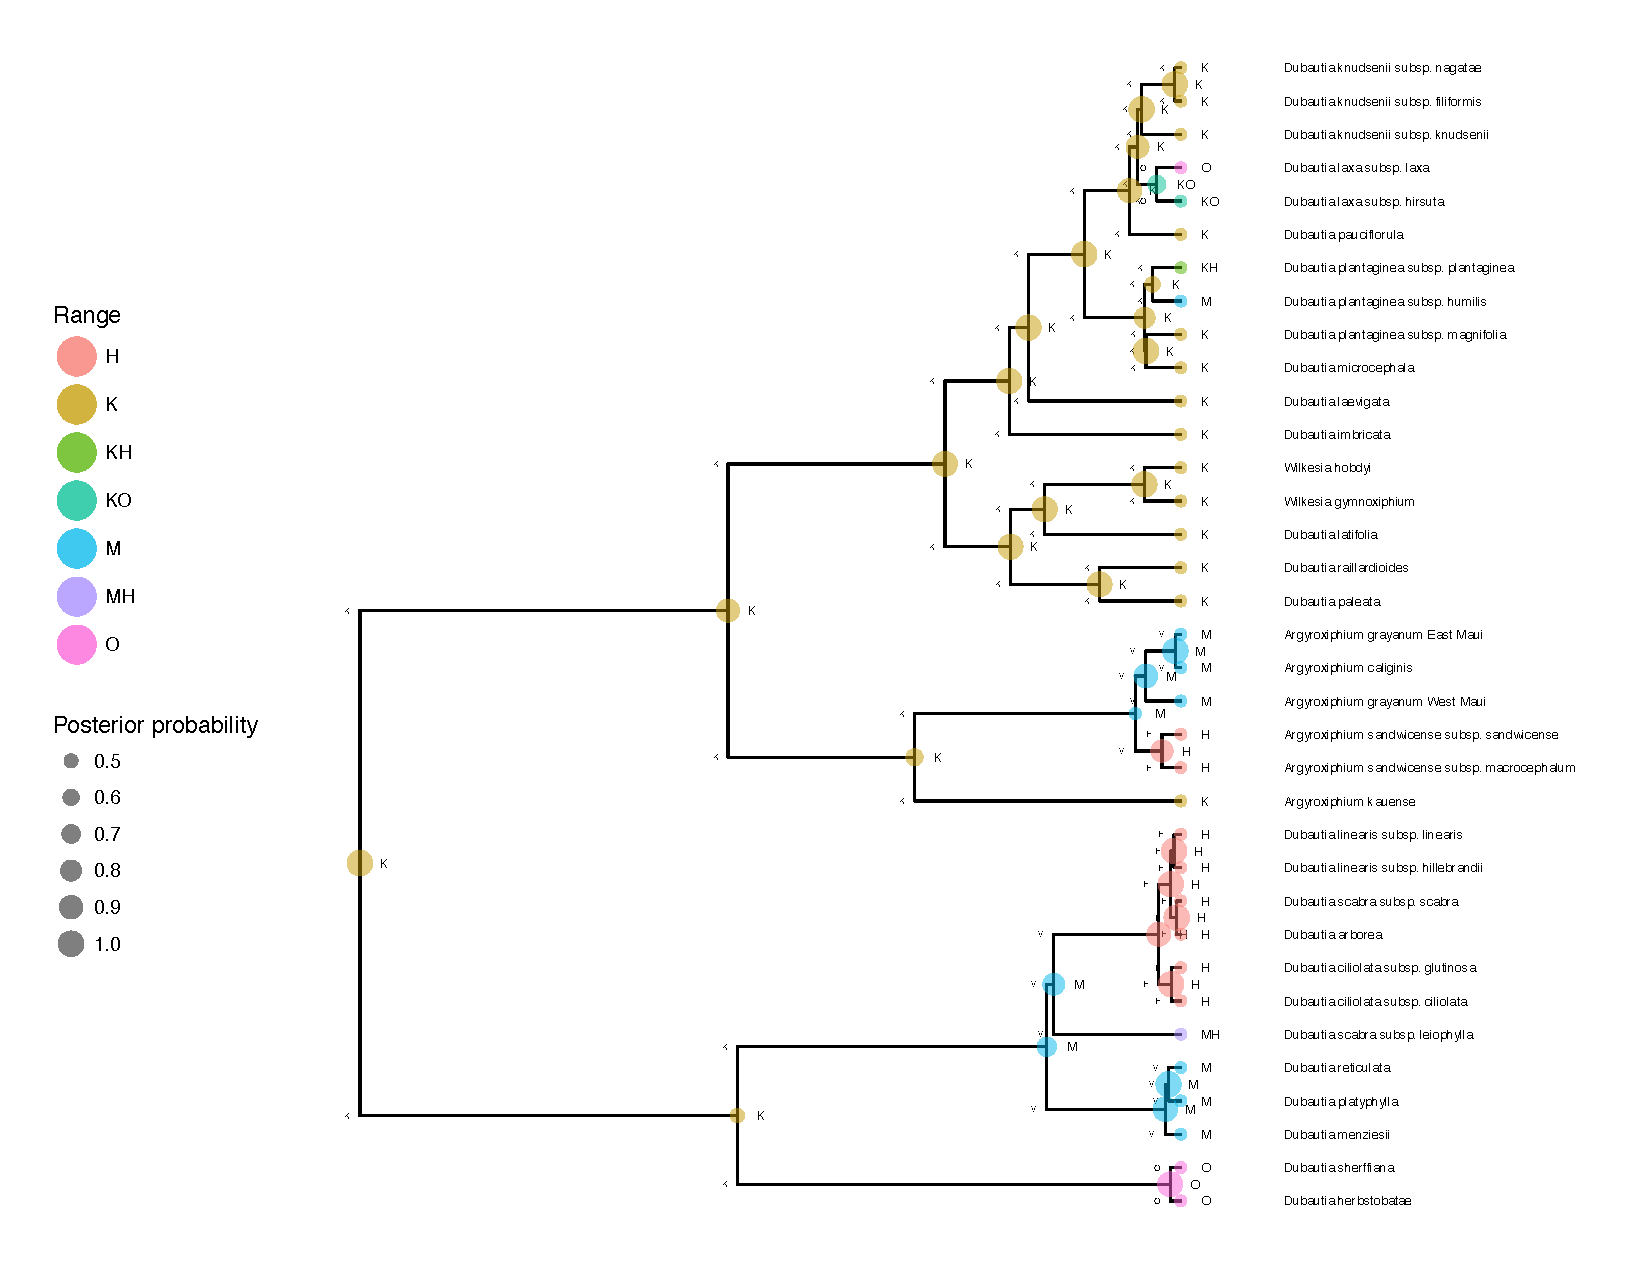
\includegraphics[width=0.7\textwidth]{figures/fig_epoch_RevGadgets_ase.pdf}
\caption{Tree with ancestral state estimates. Nodes are annotated with ancestral states before and after cladogenetic events. Most probable states are shown. Colors of markers indicate the range state. Sizes of markers indicate the posterior probability of that state. }
\label{fig:epoch_RevGadgets_ase}
\end{figure}

[ Look at posterior estimates for distance. ]

\newpage
